%!TEX root = ../Main.tex
In order to calculate the transport of electrons in NPG as well as the local density of states, LDOS, one must obtain the Green's functions and self energies related to the unit cells of the system. To do so, a recursion algorithm must be implemented as calculations become too costly for the system, even if it is small. Especially the inversion of matrices required to obtain the Green's function can be very demanding computationally, when the system contains a lot of atoms. The recursion algorithm reduces the size of the system and thereby the amount of computational time required to obtain both the first cell Green's function, the Green's function within the chain (of repeated unit cells) sometimes called \(\mathbf{G}_{bulk}\) as well as the self energies related to those Green's functions. The recursion works by utilising that one can remove every second cell in an infinite chain of cells. As the chain originally was infinite, removing every second cell will just yield a new infinite chain. Every cell has with it, its hopping matrices and Hamiltonian. The removal of every second cell is iterated, changing the effective interaction between the cells and thus the hopping matrices as well as the Hamiltonians of the system. In the end the recursion algorithm produces re-normalised Hamiltonians and hopping matrices, which can be used to obtain the Green's functions and self energies.
\subsubsection{Obtaining first cell self energy and Green's function for a simple four-atom system}\label{recursionroutinesec}
For simplicity and in order to check whether the routine would yield the results expected, the starting point is a simple system containing only 4 atoms in the unit cell (See \cref{appfigs}, \cref{Testcell}). The idea is to make a function that takes in an energy, a Hamiltonian (alternatively two in case there is a special site in the molecule) and a hopping matrix as arguments and in turn outputs the Green's function as well as the self energies going left and right. Firstly all the necessary variables are defined. The first of these consists of a complex number matrix which has the value \(E + i\eta\) in the diagonal and dimension identical to that of the Hamiltonian given as argument (in the case of the four-atom system a 4x4). Here \(E\) is the energy which the function takes as an argument as well as \(\eta\) which is a small number (in this specific case \(1\times10^{-6}\)). Note that \(\eta\) should not be made too small as it will yield incorrect results. Generally one should adjust \(\eta\) until a satisfying result have been obtained. The rest of the variables are the Hamiltonian, hopping matrices and Green's function. They are defined as: \(a0 = V^{\dagger}, \ b0 = V, \ e0_{s} = h_s, \ e_{0} = h, \ g0 = (z-e0)^{-1}\). Note that the Hamiltonian \(h\), in this specific case, is the same for both \(e0_{s}\) and \(e0\) as the first cell is identical to those of the rest of the molecule. Now that the variables are defined, the actual recursion can begin. The function \textit{RecursionRoutine} has been developed. As the recursion is an algorithm that runs for an arbitrary amount of iterations, a while loop is chosen to run the iterations until a threshold has been reached. In \cref{recurfunc} the code for the routine is shown. Line 64-70 is the listing of variables, 71-78 is the while loop with the matrix multiplication, 80-84 is the redefinition of new variables in terms of the old and 86-89 is the definition of the outputs as per \cref{outputs}.\\
\newpage
\im{Listings/Functions.py}{62}{89}
\vspace{-1\baselineskip}
\captionof{listing}{The while loop in the recursion routine. The matrix elements are overwritten with the new variables until the resulting matrix is small enough to diagonalise\label{recurfunc}}\vspace{\baselineskip}\newpage
The threshold is defined as the absolute maximum value element in the hopping matrix \(a0\) approaches zero. In this specific case it was set to \(1\times10^{-8} \). However, the value should be adjusted so that it is optimised for the specific system on which the calculation are made. Within this while loop a range matrix multiplications are computed. These constitutes the actual recursion and their order are of big importance for a correct result. Notice, however, that the code (\cref{recurfunc}) contains intermediate products of \(a0, b0\) and \(g0\). This is for run time optimisation. Following is a list of these matrix products:
\begin{align*}
	a1     & = a0 \times g0 \times a0                   \\
	b1     & = b0\times g0\times b0                   \\
	e1     & = e0 + a0\times g0\times b0 + b0\times g0\times a0 \\
	e1_{s} & = e0_{s} + a0\times g0\times b0          \\
	g1     & = (z - e1)^{-1}
\end{align*}
As stated above in the equations, the matrix product are defined as new variables with a \(+1\) variable name. This is all very well but the while loop would stop here because of the definition of new variables. It is therefore necessary to redefine the new variables in terms of the old ones (f.ex. \(a0 = a1\)) (see \cref{recurfunc} line 78-82) an as such the while loop will continue until the threshold has been reached. For the rest of the function the only thing left to do is to define the self energies and the first cell Green's function using the variables obtained from the while loop. These are simply given as:
\begin{align}\label{outputs}
	\mathbf{\Sigma}_R & = e_s - h                   \\ \nonumber
	\mathbf{\Sigma}_L & = e - h - \mathbf{\Sigma}_R \\ \nonumber
	\mathbf{G00}      & = (z - e_s)^{-1}
\end{align}
Where \(e_s\) and \(e\) are the resulting matrices from the while loop (\(e0_s, e0\)). The first cell Green's function as well as the self energies has now been obtained by recursion.
\subsubsection{Plotting the real and imaginary part of the first cell Green's function}
As a good way to check whether the recursion routine has been implemented successfully, the real and imaginary part of the Green's function can be plotted. In addition these plots gives valuable information about the local density of states at specific sites in the molecule. With a relatively simple approach, the Green's function can be obtained as a function of energy, using a \textit{for loop}, looping over a range of energies which is then used as input in the \textit{RecursionRoutine} function (\cref{recurfunc}), see \cref{plotcode}:
\im{Listings/SelfEnergyByRecursion.py}{64}{68}
\vspace{-1\baselineskip}
\captionof{listing}{Code showing the loop which produces the Green's function (or y) values for a range of energies used in the plot.\label{plotcode}}\vspace{\baselineskip}
The output from this loop will be the complex y-values for the plot. These will have to be sorted to imaginary and real parts before plotting. The x-values will just be the energy range used for the loop. The imaginary, it represents the local density of states LDOS. Note that the plot only represents the LDOS for a specific site on the molecule and that they change radically from site to site (see \cref{appfigs}, \cref{siteLDOSplot} for an example using the same structure as \cref{interface}). The site can be changed by choosing another index in \cref{plotcode} line 68, which corresponds to the atom indices in \cref{Testcell}. A plot of the real and imaginary part of the first cell Green's function (index 0) obtained by the recursion routine for the simple four-atom unit cell described in \cref{recursionroutinesec} is shown in \cref{imrealplot}.
\begin{figure}
	\centering
	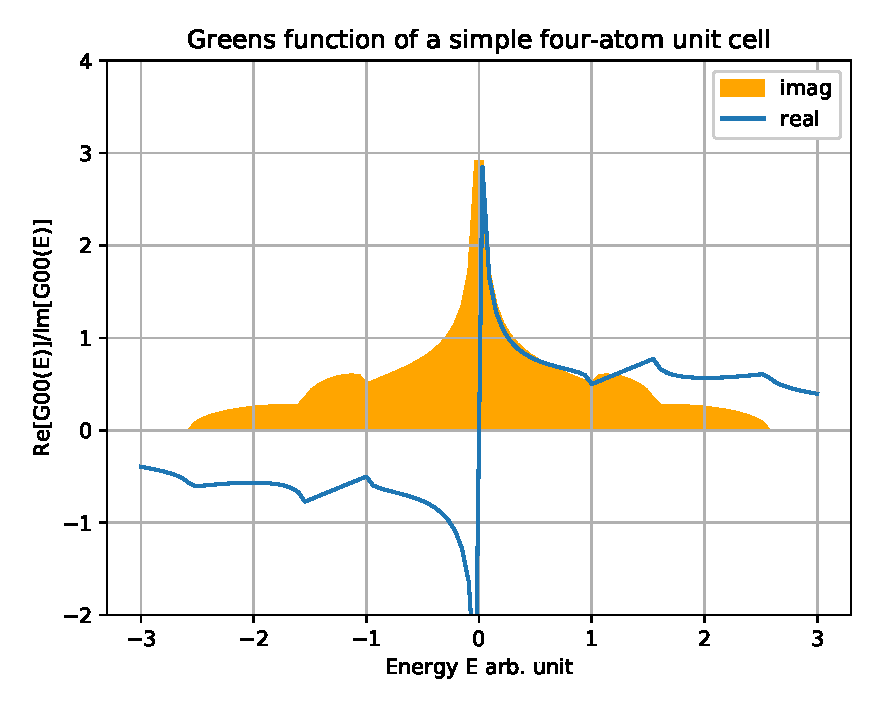
\includegraphics[width = 0.5\textwidth]{Figures/imrealplot.eps}
	\caption{A plot showing the real and imaginary part of the first cell Green's function resulting from the recursion routine on the simple system. Note that the yellow imaginary part is the representation of the local density of states.}
	\label{imrealplot}
\end{figure}
